%\documentclass{scrartcl}
%\usepackage{newclude}
%\usepackage{../Header}
%\usepackage{../../Header}
%\usepackage{../../../Header}
%\begin{document}

%\HeaderDoc{Rechnersysteme und Netze}{WS10/11}{Stephan Heidinger}{RSN Zusammenfassung}{V 0.5}{Zusammenfassung Rechnersysteme und -netze}

\documentclass{scrartcl}

\usepackage{Header}

%\usepackage{scalefnt}
%\usepackage{parcolumns}
%\usepackage{tikz-er2}
\usepackage{hyperref}

\begin{document}

\Gruppe{Stephan Heidinger}{RSN - Zusammenfassung, V 0.6}
\Header{Rechnersysteme}{Wintersemester 2010/2011}{Stephan Heidinger}{}%leave last variable empty, else there will be aufgabenblatt überschrift

\begin{shaded}
Dieses Dokument wurde unter der Creative Commons - Namensnennung-NichtKommerziell-Weitergabe unter gleichen Bedingungen (\textbf{CC by-nc-sa}) veröffentlicht. Die Bedingungen finden sich unter \href{http://creativecommons.org/licenses/by-nc-sa/3.0/de}{diesem Link}. \\
\centerline{
\includegraphics[scale=1]{../cc-by-nc-sa.png} }
\end{shaded}

\textit{Find any errors? Please send them back, I want to keep them!}

\subsection*{Vorlesung 0 - Hardware, Einstieg}
 \begin{itemize}
 \item viel blabla...
 \item \textbf{Z3} erste elektrische Rechenmaschine 1941, Representationen von Zahlen im Binärsystem (Relais)
 \item \textbf{Additionssysteme} Einzelne Symbole haben einen Wert, die Werte werden einfach addiert, etwa \emph{Römische Zahlen} oder \emph{Unärsystem}. Vorteile: Addition sehr einfach, Nachteile: andere arithmetische Operationen schwer, unübersichtlich
 \item \textbf{Stellenwertsysteme} Jedes Symbol hat einen Wert, jede Stelle hat einen Wert, der Wert der gesamten Zahl setzt sich zusammen aus der Summe der Werte jedes Symboles multipliziert mit dem Wert der Stelle (Basis hoch Stellennummer) Vorteile: Einfache arithmetische Operationen möglich.
 \item \textbf{Systeme zur Darstellung des Binärsystems:} Binärsystem schnell unübersichtlich \\
  \emph{Oktal:} Basis $8=2^3$, eher veraltet, früher gebräuchlich, heute noch für etwa Rechte in UNIX-Systemen\\
  \emph{Dezimal:} Basis $10$, Darstellung in menschengewohnter Form \\
  \emph{Hexadezimal:} Basis $16=2^4$, kompakte Darstellung, 2 Stellen = 1 Byte
 \item Umrechnungen: \\
  \begin{tabular}{|l|l|l|}
  \hline Quell & Ziel & Algorithmus \\
  \hline 
  \hline bin & oct & 3er Gruppierung \\
  \hline bin & hex & 4er Gruppierung \\
  \hline oct & hex & erst zu bin, dann wie bin$\to$hex \\
  \hline hex & oct & erst zu bin, dann wie bin$\to$oct \\
  \hline dec & base n & Teilen mit Rest durch n bis Rest 0 \\
  \hline base n & dec & Hornerschema \\
  \hline base m & base n & Erst zu dec, dann wie dec$\to$base n \\
  \hline \end{tabular}
 \item \textbf{Zahlensysteme:} \\
  \emph{metrisch} Basis 10 (spezielle Symbole für Basis 2), SI-Einheiten, konsistent, Umrechnung, basiert auf Vielfachen von Basiseinheiten\\
  \emph{imperial} Basiert auf (traditionellen) Alltagswerten (Fuß, Elle, Stein,\dots), schwer umzurechnen, wegen variierender Basis
  \item powers of 2 \\
   \begin{tabular}{c|c|c|c|c|c|c|c|c|c|c|c|c|c|c|c}
   $2^1$ & $2^2$ & $2^3$ & $2^4$ & $2^5$ & $2^6$ & $2^7$ & $2^8$ & $2^9$ & $2^{10}$ & $2^{11}$ & $2^{12}$ & $2^{13}$ & $2^{14}$ & $2^{15}$ & $2^{16}$ \\
   \hline 2 & 4 & 8 & 16 & 32 & 64 & 128 & 256 & 512 & 1024 & 2048 & 4096 & 8192 & 16384 & 32768 & 65536
   \end{tabular}
 \end{itemize}

\subsection*{Vorlesung 1 - Hardware}
 \begin{itemize}
 \item Geschwindigkeitssteigerung
  \begin{description}
   \item[processor speed:] mehr Speed im Prozessor $\Rightarrow$ mehr Gesamtspeed
   \item[component size:] kleinere Komponenten $\Rightarrow$ kürzere Wege $\Rightarrow$ schneller
   \item[memory size:] memory speed nimmt kaum zu
   \item[optimization of structure:] pipelining (fetch, decode, execute gleichzeitig), speculative execution, parallel/redundant units (>1 apu, multiple cores, multithreading,\dots)
  \end{description}
  \item \textbf{Moore's Law} \emph{The number of transistors on given chip area doubles every 18 months.}
  \item \textbf{Computer Architecture} Von-Neumann-Rechner:
   \begin{description}
    \item[CPU] Steuer- und Rechenwerk, Steuerung der Befehlsabfolge + Rechenoperationen
    \item[Speicher] Speichert Daten und Instruktionen (Text)
    \item[I/O] in-/output + interfaces
   \end{description}
   \textbf{Nachteil:} Von-Neumann-Flaschenhals: Daten und Text über einen Bus, CPU schneller als Bus
   \item verschiedenes:
    \begin{description}
     \item[Halbleiter:] auf Silizium basierend, abhängig von Temperatur Leiter oder Isolator
     \item[Transistor:] Schalten und Verstärken elektrischer Signale
     \item[Kondensator:] speichert elektrische Energie
     \item[Integrierter Schaltkreis:] elektronische Schaltung auf einem Halbleiter
    \end{description}
   \item Speicherhirarchie
    \begin{itemize}
     \item register 
     \item  cache 
     \item  main memory 
     \item  solid state drive 
     \item  electronic disk 
     \item  magnetic disk 
     \item  optical disk 
     \item  magnetic tape 
    \end{itemize}
   \item \textbf{Betriebssystem:} Management von Prozessen, Abstraktion von Hardware (Speichermanagement, Interruptmanagement, Dateisystemmanagement, Gerätetreiber, System Calls als Abstraktion, ...)
   \item \textbf{Virtuelle Maschine:} ein aus Software bestehender Rechner, als Betriebssystem simuliert sie Hardware, als Laufzeitumgebung virtuellen Prozessor
   \item \textbf{Kernel:}
    \begin{description}
     \item[kernel space:] Speicherbereich des Kernels, Prozesse in diesem Bereich haben volle Sichtbarkeit und vollen Zugriff auf Hardware     
     \item[user space:] restlicher Speicherbereich, kein direkter Zugriff auf Resourcen
     \item[monolithischer Kernel:] alle Komponenten als ein Prozess im kernel space, Volle Sichtbarkeit, Fehler führt zu system failure (Linux/UNIX, DOS, Windows (ohne NT), OS/2)
     \item[Mkcrokernel:] Nur wichtigste Prozesse (Prozesskommunikation, Speicher-/Prozessmanagement) im kernel space, Fehler lässt nur einzelne Komponenten abstürzen, hoher Aufwand für Synchronisation (minix, Mach, Hurd, QNX)
     \item[Hybridkernel:] Mischung aus monolitisch und mikro (Windows NT, XNU/Darwin/OSx)
    \end{description}
 \end{itemize}
 
\subsection*{Vorlesung 2 - File System, Operating System, Process Management}
 \begin{itemize}
 \item \textbf{File System:} Abstrahiert I/O Geräte, Dateien als Geräte unabhängige Entitäten, organisiert Daten in Dateien und Vereichnissen, sicher Integrität und Zugriff, managed Speicher
 \item \textbf{File System}\\
  Main Memory/RAM (random access memory), CPU can access directly, volatile \\
  Secondary Storage, non-volatile, large, slower\\
  \begin{tabular}{|cllr||cllr|}
  \hline
  k & kilo & $10^3$ & 1\;000 & Ki & kibi & $2^{10}$ & 1\;024 \\
  M & mega & $10^6$ & 1\;000\;000 & Mi & mebi & $2^{20}$ & 1\;048\;576 \\
  G & giga & $10^9$ & 1\;000\;000\;000 & Gi & gibi & $2^{30}$ & 1\;073\;741\;824 \\
  T & tera & $10^{12}$ & 1\;000\;000\;000\;000 & Ti & tebi & $2^{40}$ & 1\;099\;511\;627\;776 \\
  \hline
  \end{tabular}
  \item \textbf{read/write-delay:} seek time (move heads to track, wait for head to settle), rotational delay (wait for sector to move under head), transfer time (read/write time) \\
  access time = seek time + rotational delay + transfer time \\
  $\displaystyle\text{transfer time} = \frac{\text{transferrate}}{\text{blocksize}}$ \\
  $\text{capacity} = \text{cylinders} \cdot \text{heads}\cdot \text{sectors}\cdot \text{sector size}$ \\
  $\displaystyle\text{cylinders}=\frac{\text{tracks}}{\text{side}}$
  \item \textbf{File System Requirements:} Block allocation/management/caching, Name/file mapping (list, open, close), File offset/block mapping (read, write, seek), Access Control 
  \item \textbf{SSD/Solid State Drive:} Halbleiterspeicher, keine mechanischen Teile $\Rightarrow$ leiser, schneller, robuster, energieeffizienter, ABER: teuer, weniger Kapazität, schwierige Herstellung
  \item \textbf{MBR/Master Boot Record:} 1 Block (512B) Bootloader und Partitionstabelle
  \item \textbf{DOS/FAT:} (file allocation table) Drive Letters, Special Devices, Sequential Files \\
  Gleich große Cluster, FAT hat für jeden Eintrag einen Cluster
  Disk Layout:
  \begin{itemize}
  \item boot block
  \item file allocation tables
  \item root directory area
  \item data area (+directory hirarchy)
  \end{itemize}
 \textbf{VFAT:} Long File Names
 \item \textbf{Fragmentierung:} Verstreutes Speichern zusammengehörender Daten, Verhindern durch: Defragmentieren, grössere Blöcke, preallokation von Blöcken, spätes Festlegen von Blöcken
 \item \textbf{Inodes}: UNIX-Idee, Baumstruktur
 \item \textbf{Betriebssystem:} wimp: \underline{w}indow, \underline{i}con, \underline{m}enu, \underline{p}ointer
 \item \textbf{Processes:} programm vs process \\
 % Graphic for TeX using PGF
% Title: F:\home\My Dropbox\UniWork\Übungen\RSN\Übungsblatt 3\RSNB7\life-cycle.dia
% Creator: Dia v0.97.1
% CreationDate: Tue Feb 08 00:38:13 2011
% For: Pandora
% \usepackage{tikz}
% The following commands are not supported in PSTricks at present
% We define them conditionally, so when they are implemented,
% this pgf file will use them.
\ifx\du\undefined
  \newlength{\du}
\fi
\setlength{\du}{15\unitlength}
\begin{tikzpicture}
\pgftransformxscale{1.000000}
\pgftransformyscale{-1.000000}
\definecolor{dialinecolor}{rgb}{0.000000, 0.000000, 0.000000}
\pgfsetstrokecolor{dialinecolor}
\definecolor{dialinecolor}{rgb}{1.000000, 1.000000, 1.000000}
\pgfsetfillcolor{dialinecolor}
\definecolor{dialinecolor}{rgb}{1.000000, 1.000000, 0.000000}
\pgfsetfillcolor{dialinecolor}
\pgfpathellipse{\pgfpoint{19.450000\du}{6.150000\du}}{\pgfpoint{3.450000\du}{0\du}}{\pgfpoint{0\du}{2.150000\du}}
\pgfusepath{fill}
\pgfsetlinewidth{0.100000\du}
\pgfsetdash{}{0pt}
\pgfsetdash{}{0pt}
\definecolor{dialinecolor}{rgb}{0.000000, 0.000000, 0.000000}
\pgfsetstrokecolor{dialinecolor}
\pgfpathellipse{\pgfpoint{19.450000\du}{6.150000\du}}{\pgfpoint{3.450000\du}{0\du}}{\pgfpoint{0\du}{2.150000\du}}
\pgfusepath{stroke}
% setfont left to latex
\definecolor{dialinecolor}{rgb}{0.000000, 0.000000, 0.000000}
\pgfsetstrokecolor{dialinecolor}
\node at (19.450000\du,6.372500\du){wartend};
\definecolor{dialinecolor}{rgb}{0.000000, 1.000000, 0.000000}
\pgfsetfillcolor{dialinecolor}
\pgfpathellipse{\pgfpoint{15.500000\du}{17.720000\du}}{\pgfpoint{3.450000\du}{0\du}}{\pgfpoint{0\du}{2.150000\du}}
\pgfusepath{fill}
\pgfsetlinewidth{0.100000\du}
\pgfsetdash{}{0pt}
\pgfsetdash{}{0pt}
\definecolor{dialinecolor}{rgb}{0.000000, 0.000000, 0.000000}
\pgfsetstrokecolor{dialinecolor}
\pgfpathellipse{\pgfpoint{15.500000\du}{17.720000\du}}{\pgfpoint{3.450000\du}{0\du}}{\pgfpoint{0\du}{2.150000\du}}
\pgfusepath{stroke}
% setfont left to latex
\definecolor{dialinecolor}{rgb}{0.000000, 0.000000, 0.000000}
\pgfsetstrokecolor{dialinecolor}
\node at (15.500000\du,17.942500\du){Erstellung};
\definecolor{dialinecolor}{rgb}{1.000000, 0.000000, 0.000000}
\pgfsetfillcolor{dialinecolor}
\pgfpathellipse{\pgfpoint{23.050000\du}{17.770000\du}}{\pgfpoint{3.450000\du}{0\du}}{\pgfpoint{0\du}{2.150000\du}}
\pgfusepath{fill}
\pgfsetlinewidth{0.100000\du}
\pgfsetdash{}{0pt}
\pgfsetdash{}{0pt}
\definecolor{dialinecolor}{rgb}{0.000000, 0.000000, 0.000000}
\pgfsetstrokecolor{dialinecolor}
\pgfpathellipse{\pgfpoint{23.050000\du}{17.770000\du}}{\pgfpoint{3.450000\du}{0\du}}{\pgfpoint{0\du}{2.150000\du}}
\pgfusepath{stroke}
\definecolor{dialinecolor}{rgb}{0.847059, 0.898039, 0.898039}
\pgfsetfillcolor{dialinecolor}
\pgfpathellipse{\pgfpoint{27.000000\du}{11.720000\du}}{\pgfpoint{3.450000\du}{0\du}}{\pgfpoint{0\du}{2.150000\du}}
\pgfusepath{fill}
\pgfsetlinewidth{0.100000\du}
\pgfsetdash{}{0pt}
\pgfsetdash{}{0pt}
\definecolor{dialinecolor}{rgb}{0.000000, 0.000000, 0.000000}
\pgfsetstrokecolor{dialinecolor}
\pgfpathellipse{\pgfpoint{27.000000\du}{11.720000\du}}{\pgfpoint{3.450000\du}{0\du}}{\pgfpoint{0\du}{2.150000\du}}
\pgfusepath{stroke}
% setfont left to latex
\definecolor{dialinecolor}{rgb}{0.000000, 0.000000, 0.000000}
\pgfsetstrokecolor{dialinecolor}
\node at (23.050000\du,17.992500\du){Beendigung};
% setfont left to latex
\definecolor{dialinecolor}{rgb}{0.000000, 0.000000, 0.000000}
\pgfsetstrokecolor{dialinecolor}
\node at (27.000000\du,11.942500\du){laufend};
\definecolor{dialinecolor}{rgb}{1.000000, 1.000000, 0.000000}
\pgfsetfillcolor{dialinecolor}
\pgfpathellipse{\pgfpoint{12.450000\du}{11.870000\du}}{\pgfpoint{3.450000\du}{0\du}}{\pgfpoint{0\du}{2.150000\du}}
\pgfusepath{fill}
\pgfsetlinewidth{0.100000\du}
\pgfsetdash{}{0pt}
\pgfsetdash{}{0pt}
\definecolor{dialinecolor}{rgb}{0.000000, 0.000000, 0.000000}
\pgfsetstrokecolor{dialinecolor}
\pgfpathellipse{\pgfpoint{12.450000\du}{11.870000\du}}{\pgfpoint{3.450000\du}{0\du}}{\pgfpoint{0\du}{2.150000\du}}
\pgfusepath{stroke}
% setfont left to latex
\definecolor{dialinecolor}{rgb}{0.000000, 0.000000, 0.000000}
\pgfsetstrokecolor{dialinecolor}
\node at (12.450000\du,12.092500\du){bereit};
\pgfsetlinewidth{0.100000\du}
\pgfsetdash{}{0pt}
\pgfsetdash{}{0pt}
\pgfsetbuttcap
{
\definecolor{dialinecolor}{rgb}{0.000000, 0.000000, 0.000000}
\pgfsetfillcolor{dialinecolor}
% was here!!!
\pgfsetarrowsend{stealth}
\definecolor{dialinecolor}{rgb}{0.000000, 0.000000, 0.000000}
\pgfsetstrokecolor{dialinecolor}
\draw (14.410980\du,15.631224\du)--(13.539020\du,13.958776\du);
}
\pgfsetlinewidth{0.100000\du}
\pgfsetdash{}{0pt}
\pgfsetdash{}{0pt}
\pgfsetbuttcap
{
\definecolor{dialinecolor}{rgb}{0.000000, 0.000000, 0.000000}
\pgfsetfillcolor{dialinecolor}
% was here!!!
\pgfsetarrowsend{stealth}
\definecolor{dialinecolor}{rgb}{0.000000, 0.000000, 0.000000}
\pgfsetstrokecolor{dialinecolor}
\pgfpathmoveto{\pgfpoint{14.654376\du}{13.573217\du}}
\pgfpatharc{120}{59}{10.075245\du and 10.075245\du}
\pgfusepath{stroke}
}
\pgfsetlinewidth{0.100000\du}
\pgfsetdash{}{0pt}
\pgfsetdash{}{0pt}
\pgfsetbuttcap
{
\definecolor{dialinecolor}{rgb}{0.000000, 0.000000, 0.000000}
\pgfsetfillcolor{dialinecolor}
% was here!!!
\pgfsetarrowsend{stealth}
\definecolor{dialinecolor}{rgb}{0.000000, 0.000000, 0.000000}
\pgfsetstrokecolor{dialinecolor}
\pgfpathmoveto{\pgfpoint{24.703522\du}{10.071520\du}}
\pgfpatharc{298}{241}{10.469220\du and 10.469220\du}
\pgfusepath{stroke}
}
\pgfsetlinewidth{0.100000\du}
\pgfsetdash{}{0pt}
\pgfsetdash{}{0pt}
\pgfsetbuttcap
{
\definecolor{dialinecolor}{rgb}{0.000000, 0.000000, 0.000000}
\pgfsetfillcolor{dialinecolor}
% was here!!!
\pgfsetarrowsend{stealth}
\definecolor{dialinecolor}{rgb}{0.000000, 0.000000, 0.000000}
\pgfsetstrokecolor{dialinecolor}
\pgfpathmoveto{\pgfpoint{26.598855\du}{9.534491\du}}
\pgfpatharc{339}{288}{5.779222\du and 5.779222\du}
\pgfusepath{stroke}
}
\pgfsetlinewidth{0.100000\du}
\pgfsetdash{}{0pt}
\pgfsetdash{}{0pt}
\pgfsetbuttcap
{
\definecolor{dialinecolor}{rgb}{0.000000, 0.000000, 0.000000}
\pgfsetfillcolor{dialinecolor}
% was here!!!
\pgfsetarrowsend{stealth}
\definecolor{dialinecolor}{rgb}{0.000000, 0.000000, 0.000000}
\pgfsetstrokecolor{dialinecolor}
\pgfpathmoveto{\pgfpoint{16.105139\du}{6.793793\du}}
\pgfpatharc{245}{208}{6.584505\du and 6.584505\du}
\pgfusepath{stroke}
}
\pgfsetlinewidth{0.100000\du}
\pgfsetdash{}{0pt}
\pgfsetdash{}{0pt}
\pgfsetbuttcap
{
\definecolor{dialinecolor}{rgb}{0.000000, 0.000000, 0.000000}
\pgfsetfillcolor{dialinecolor}
% was here!!!
\pgfsetarrowsend{stealth}
\definecolor{dialinecolor}{rgb}{0.000000, 0.000000, 0.000000}
\pgfsetstrokecolor{dialinecolor}
\draw (25.672565\du,13.753160\du)--(24.377435\du,15.736840\du);
}
% setfont left to latex
\definecolor{dialinecolor}{rgb}{0.000000, 0.000000, 0.000000}
\pgfsetstrokecolor{dialinecolor}
\node[anchor=west] at (17.150000\du,10.100000\du){Unterbrechung};
% setfont left to latex
\definecolor{dialinecolor}{rgb}{0.000000, 0.000000, 0.000000}
\pgfsetstrokecolor{dialinecolor}
\node[anchor=west] at (16.250000\du,14.050000\du){Scheduler/Dispatcher};
% setfont left to latex
\definecolor{dialinecolor}{rgb}{0.000000, 0.000000, 0.000000}
\pgfsetstrokecolor{dialinecolor}
\node[anchor=west] at (26.200000\du,6.900000\du){I/O};
% setfont left to latex
\definecolor{dialinecolor}{rgb}{0.000000, 0.000000, 0.000000}
\pgfsetstrokecolor{dialinecolor}
\node[anchor=west] at (26.200000\du,7.700000\du){Warten auf Aktion};
% setfont left to latex
\definecolor{dialinecolor}{rgb}{0.000000, 0.000000, 0.000000}
\pgfsetstrokecolor{dialinecolor}
\node[anchor=west] at (26.200000\du,8.500000\du){...};
% setfont left to latex
\definecolor{dialinecolor}{rgb}{0.000000, 0.000000, 0.000000}
\pgfsetstrokecolor{dialinecolor}
\node[anchor=east] at (13.900000\du,6.850000\du){I/O};
% setfont left to latex
\definecolor{dialinecolor}{rgb}{0.000000, 0.000000, 0.000000}
\pgfsetstrokecolor{dialinecolor}
\node[anchor=east] at (13.900000\du,7.650000\du){Aktion beendet};
% setfont left to latex
\definecolor{dialinecolor}{rgb}{0.000000, 0.000000, 0.000000}
\pgfsetstrokecolor{dialinecolor}
\node[anchor=east] at (13.900000\du,8.450000\du){...};
% setfont left to latex
\definecolor{dialinecolor}{rgb}{0.000000, 0.000000, 0.000000}
\pgfsetstrokecolor{dialinecolor}
\node[anchor=west] at (12.050000\du,15.600000\du){admit};
% setfont left to latex
\definecolor{dialinecolor}{rgb}{0.000000, 0.000000, 0.000000}
\pgfsetstrokecolor{dialinecolor}
\node[anchor=west] at (25.550000\du,15.200000\du){exit};
\end{tikzpicture}
 \\
 PCB (process control block), contains necessary information to: interrupt/continue, remember I/Os and file usage of process, remember privileges (Eintrag in Prozesstabelle, Status, program counter, stack pointer, singals, scheduling info, \dots\\
 forking of processes
 \item \textbf{Scheduler:} allow processes to use cpu, while other processes waiting, Gannt-charts, models:
  \begin{description}
  \item[FCFS:] First Come, First Serve
  \item[(P)SJF:] (Preemtive) Shortest Job First
  \item[PHPF:] Preemtive Highest Priority First
  \item[preemptive] (interrupt running task for one with higher priority)
  \item[EWMA:] Exponentially Weighted Moving Average, tries to calculate CPU burst times via past bursts, older bursts are less weighted
  \item[round robin:] gewährt Prozessen in einem Ringverfahren jeweils kurze Zeitschlitze
  \end{description}
  \item \textbf{Protection:} Kernel/User mode, memory protection (process cant write outside its allocated memory
 \end{itemize}
 
\subsection*{Vorlesung 3 - Assembler}
 \begin{itemize}
 \item \textbf{Assembler} \emph{mnemonics} $\to$ machine language, down to the roots, incredibly fast (airbag, brake control, \dots \\
  \begin{tabular}{|ll|}
  \hline Opcode & Operation \\
  \hline add r, a, b & r $\leftarrow$ a+b \\
  sub r, a, b & r $\leftarrow$ a-b \\
  mul r, a, b & r $\leftarrow$ a*b \\
  div r, a, b & r $\leftarrow$ a/b \\
  mod r, a, b & r $\leftarrow$ a\%b \\
  neg r, a    & r $\leftarrow$ -a \\
  sign r, a   & r $\leftarrow$ signof(a)$\lbrace -1,0,+1 \rbrace$ \\
  abs r, a    & r $\leftarrow$ $\vert a\vert \equiv r \leftarrow a\cdot$ signof(a)\\
  mov r, a    & r $\leftarrow$ a \\
  set const, cexpr & $\leftarrow$ define constant $const$ \\
  and r, a, b & r $\leftarrow$ $a\land b$ \\
  or r, a, b  & r $\leftarrow$ $a \lor b$ \\
  xor r, a, b & r $\leftarrow$ $a \oplus b$ \\
  not r, a    & r $\leftarrow$ $\neg a$ (logical) \\
  cmnt r, a   & r $\leftarrow$ $\neg a$ (bitwise) \\
  shr r, a, b & r $\leftarrow$ $a\gg b$ \\
  shl r, a, b & r $\leftarrow$ $a\ll b$ \\
  call label  & PC $\leftarrow$ label \\
  jmp label   & PC $\leftarrow$ label \\
  brcmp OP, label, a, b & PC $\leftarrow$ label, if a OP b \\
  brtst OP, label, a & PC $\leftarrow$ label, if a OP 0 \\
  cmp OP, r, a, b & r $\leftarrow$ (a OP b) \\
  tst OP, r, a & r $\leftarrow$ (a OP 0) \\
  stop a      & stop if a $\neq$ 0 \\
  \hline
  \end{tabular}
  \begin{tabular}{|ll|}
  \hline Operator & (OP) \\
  \hline
  LT & < \\
  GT & > \\
  LTEQ & <= \\
  GTEQ & >= \\
  EQ & == \\
  NEQ & != \\
  \hline
  \end{tabular} \\ \\
  \texttt{push} / \texttt{pop} used for stack access \\
  Auf jeden Fall bei der Assembler-Aufgabe reinschreiben...
  \ladeJava{Assembler}
  \item
   \begin{description}
    \item[Programm:] ausführbare Binärdatei, Folge von Anweisungen
    \item[Prozess:] Instanz eines Programms, Programm in Ausführung
    \item[Thread:] kleinste auszuführende Einheit (im gleichen Speicherbereich wie Prozess)
    \item[Zombie:] nicht ordnungsgemäß beendeter Prozess (Eintrag in Prozesstabelle)
    \item[Dämon:] Prozess im Hintergrund, keine Benutzerinteraktion
    \item[Verhungern:] Prozess bekommt nie die Resourcen, die er benötigt, um ausgeführt zu werden
    \item[Prozessmanager:] Multiprogramming/Multitasking/IPC (interprocess communication), minimize waiting and response time, maximize CPU usage
   \end{description}
 \end{itemize}
 
\subsection*{Vorlesung 4 - Data Encoding}
 \begin{itemize}
  \item common memory sizes: \\
   \begin{tabular}{ll}
    4 bits & nibble \\
    8 bits & byte \\
    16 bits & half word, word, short, int \\
    32 bits & word, dword, int, long \\
    64 bits & long, long long
   \end{tabular}
  \item Historic: Morse, Baudot, Telex, SIXBIT
  \item \textbf{ASCII} (American Standard Code for Information Interchange, memory efficient, no support for other languages \\
   7 bits + 1 bit checksum \\
   country specific versions (ISO 646)
  \item \textbf{ISO 8859} ASCII + extended control characters + nbsp + more printables, 15 different versions
  \item \textbf{UNICODE}: code points for all "'usefull characters "', 17 "'planes"' of 65536 code points, character = glyph (pixel-adressable display/printer)\\
  NFC: composed (U+00fc: ü) vs NFD: decomposed (U+0075: u + U+0308 \"{})
  \item \textbf{UTF-8} most common, most complex, variable length, ascii compatbile, efficient for most languages \\
   \begin{tabular}{|lcl|}
   \hline
   U+0000\dots U+007f ($\leq$ 7 bits) & $\to$ & $0xxx\;xxxx_2$ \gruen{ASCII kompatibel} \\
   U+0080\dots U+07ff (8\dots 11 bits) & $\to$ & $110x\;xxxx_2\;10xx\;xxx_2$ \\
   U+0800\dots U+ffff (12\dots 16 bits) & $\to$ & $1110\;xxxx_2\;10xx\;xxxx_2\;10xx\;xxxx_2$ \\
   U+0001\;0000\dots U+0010\;ffff (17\dots 20.1 bits) & $\to$ & $1111\;0xxx_2\;10xx\;xxx_2\;10xx\;xxxx_2\;10xx\;xxxx_2$ \\
   \hline
   \end{tabular}
  \item \textbf{UTF-16} common code points: U+0000\dots U+D7FF, U+E000\dots U+FFFF direct (U+D800\dots U+DFFF forbidden), 16 Bit für normale Zeichen, für seltene Zeichen zwei 16 surrogate bit pairs \\
  for code points U+10000 and beyond, substract U+10000, result fits into 20 bit, split in halves, Upper half with U+D800 stored first, Lower half with U+DC00 stored second \\
  BOM start file with FEFF (big endian) or FFFE (little endian)
  \item \textbf{UTF-32} fixed-length encoding
  \item \textbf{Numbers}
   \begin{itemize}
    \item \textbf{unsigned integers:} 0\dots 65\;535
    \item \textbf{sign-magnitude:} bei Hälfte des Bereichs beginnt negativer Bereich
    \item \textbf{Einerkomplement:} ein Bit zum negativieren der Zahlen
    \item \textbf{Zweierkomplement:} wie Einerkomplement, nur dass neg bei -1 startet, Addition und Substraktion sind konsistent
    \item \textbf{floating point} IEEE754 and IEEE854, 32 bit (single precision) or 64 bit (double precision) \\
    $\underset{1 bit}{\rot{S}}\underset{8 bits}{\gruen{EEEEEEEE}}\underset{23 bits}{\blau{MMMMMMMMMMMMMMMMMMMMMMM}}$ \\
    $\text{value} = \rot{(-1)^s}\cdot\blau{1.MMMMMMMMMMMMMMMMMMMMMMM}\cdot 2^{\gruen{EEEEEEEE-127}}$ \\
   \end{itemize}
 \end{itemize}
 
\subsection*{Vorlesung 5 - Digital Logic}
 \begin{itemize}
  \item Logic gates are atomary elements in modern circuits \\
   \begin{tabular}{|lcccl|}
    \hline 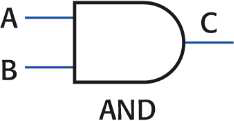
\includegraphics[scale=0.6]{logic-and.png}  & A AND B & A $\land$ B & A $\cdot$ B & Konjunktion \\
    \hline 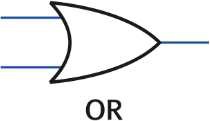
\includegraphics[scale=0.6]{logic-or.png}& A OR B  & A $\lor$ B  & A $+$ B & Disjunktion \\
    \hline 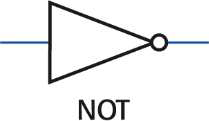
\includegraphics[scale=0.6]{logic-not.png}& NOT A   & $\neg$ A    & $\overline{\text{A}}$ & Negation \\
    \hline 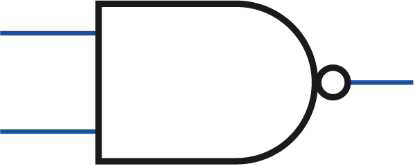
\includegraphics[scale=0.2]{logic-nand.png}& A NAND A   &    & \\
           \hline
   \end{tabular}\\
   NOT, AND, OR are functionally complete, so are NAND and NOR\\
   \begin{tabular}{|ccc|}
   \hline
   NOT A   &=& A NAND A \\
   A AND B &=& (A NAND B) NAND (A NAND B) \\
   A OR B  &=& (A NAND A) NAND (B NAND B) \\
   \hline
   \end{tabular}\\
   Multiplexers are more complex designs using $2\times n$ inputs, $n$ data lines and $n$ control lines, where always two are combined.\\
   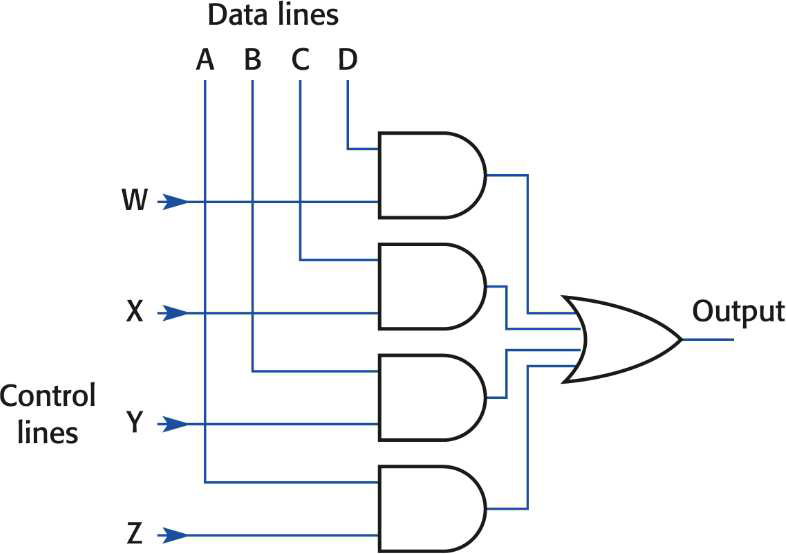
\includegraphics[scale=0.6]{logic-multiplexer.png}
  \item \textbf{sum-of-products:} find where output is 1, connect corresponding inputs via and, connect and-groups via or; DNF
  \item \textbf{product-of-sums:} find where output is 0, connect inputs via and and negate groups, connect resulting groups via and; KNF
  \item \textbf{circuit simplification:} Use boolean laws or karnaugh maps (from one field to the next, only one value changes!) \gruen{bsp-karnaugh map einfügen}
  \item \textbf{Instruction Set Architecture:}
   \begin{description}
    \item[Instruction Set:] Menge aller von der Hardware bereitgestellten Instruktionen, Datentypen, Datenstrukturen (RISC (reduced instruction set), CISC (complete instruction set))
    \item[Mnemonic:] Lesbare Representation des Opcode
    \item[Opcode:] "`Befehl"' in Maschinensprache, Nummer des Maschinenbefehls, Representation durch Mnemonic, $\sum$Opcodes$\equiv$ Befehlssatz
    \item[Pseudo-Opcode:] kein wirklicher Opcode, wird in mehrere Operationen expandiert
    \item[heap:] gesammter Speicherbereich eines Prozesses
    \item[stack:] Speicherbereich, LIFO, Rücksprungadresse, Daten, Parameter, Rückgabewerte, \dots
   \end{description}
 \end{itemize}
 
\subsection*{Vorlesung 6 - Integer Arithmetic}
 \begin{itemize}
  \item \textbf{ALU} - Arithmetic and Logic Unit $\to$ performs binary integer arithmetic operations
  \item \textbf{FPU} - Floating Point Unit, seperarate processor in larger systems else done in software
  \item \textbf{half adder:}, two outputs (sum and carry [\"Ubertrag]) \\
  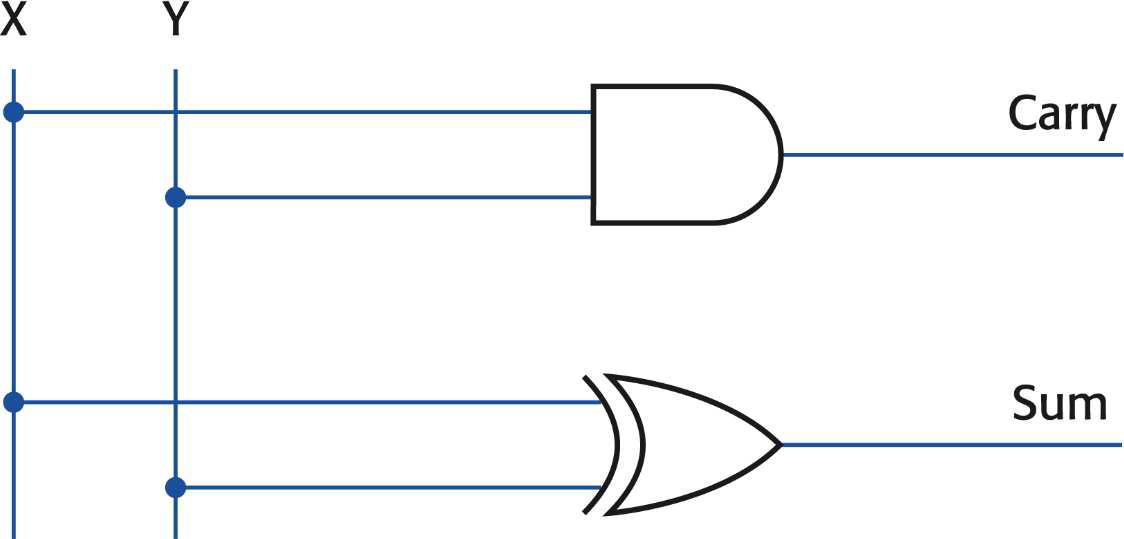
\includegraphics[scale=0.6]{arith-halfadder.png}
  \item \textbf{full Adder:} adds two bits and a carry ($Z=C_{in}$)\\
    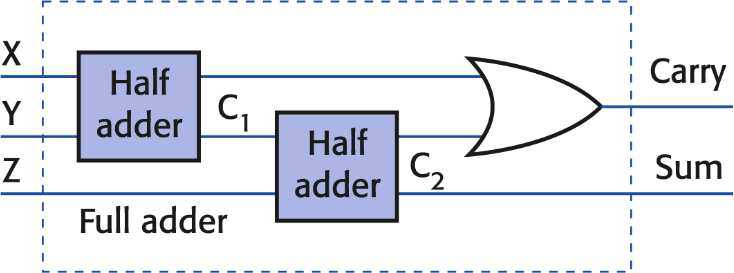
\includegraphics[scale=0.6]{arith-fulladder.png}
    \item \textbf{(parallel) n-bit adder:} assembly of full-adders\dots
    \item \textbf{(parallel) n-bit substractor:} consists of n-bit adders and negation gates and adding one (like when done by hand)
    \item \textbf{multiplication:} could be achieved by mutliple additions, but is more practical with bit-shifting techniques (like multiplication with 10 done by hand)
    \item \textbf{Flip Flop:} A flipflop has two stable states, upon signal in, one state will stay, until other input fires, \texttt{NAND}s in example can also be \texttt{NOR}s\\
    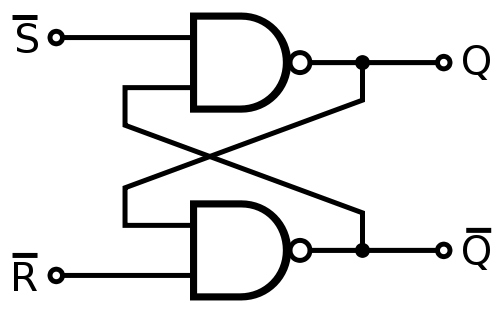
\includegraphics[scale=0.2]{arith-flipflop.png}
 \end{itemize}
 
\subsection*{Vorlesung 7 - networking intro}
 \begin{itemize}
  \item \textbf{Network:} infrastructure (hard-/software) that enables endpoins (hosts) to communicate
   \begin{description}
    \item[Frame:] data transmission or data packet with frame synchronisation (sequencing of frames)
    \item[Repeater:] amplifies \& copies any electrical signal (including noise)
    \item[Bridge:] copies frames between segments, can interpret frame data and drops frames not addressed to other segments
    \item[Router:] copies packets between segments, can interpret final destination address and has routing tables to optimize packet route
    \item[Gateway:] generic term, encompassing hardware (repeater, bridge, router) and software (router)
   \end{description}
  \item \textbf{layering} \\
   \begin{tabular}{|cp{8cm}p{6cm}|}
   \hline
   application & supporting network applications & FTP, HTTP, SMTP, POP, NNTP, IRC, STTP\\
   presentation & (OSI) representation of data, de-/encryption, machine-de/independet data & \\
   session & (OSI) Kommunikation zwischen Sitzungen von Anwendungen/Prozessen, "`interhost"' & \\
   transport & host-to-host data transfer & TCP, Ports, UDP \\
   network & path determination, logical addressing & IP, routing protocolls, IP, IPX, IPsec, Router, ARP, ICMP \\
   data/link & physical addressing & PPP, Ethernet, IEEE 802.11, Switch, Bluetooth, Modem \\
   physical & "'bits on the wire"' & cable \\
   \hline
   \end{tabular} \\ \\
   \textbf{A}ll \textbf{P}eople \textbf{S}eem \textbf{T}o \textbf{N}eed \textbf{D}ata \textbf{P}rocessing \\
   \textbf{A}lle \textbf{P}riester \textbf{S}aufen \textbf{T}equila \textbf{N}ach \textbf{D}er \textbf{P}redigt 
  \item \textbf{Internet principle:} "'We reject kings, presidents and voting. We believe in rough consensuns and running code."'\\
  \textbf{End-to-End principle} $\Rightarrow$ dumb-network, smart endpoints
  \item Berechnungen:
   \begin{description}
    \item[packet size] $p=n\cdot h[B]+d[B]=(n\cdot h+d)[B]$
    \item[gross transfer rate] $R=b[Mbps] \to R'=R\cdot \frac{10^6}{8}[Bps]$ (R is bandwidth)
    \item[package rate] $D=\frac{R'}{p}[packets/s]$
   \end{description}
  \item \textbf{TCP/IP:}
  \item \textbf{packet switching:} data is split into packets, which are sent seperately, packets carry sequence numbers, network layer uses them to fragment and reassemble packages, transport layer uses them to detect and retransmit lost packages \\
  great for "'bursty"' data \\
  excessive congestion: packet delay, loss of data
  \item \textbf{circuit switching:} i.e. telephone, direct physical link used exclusively by the communications endpoints\\
  great for constant bit rate \\
  no resource sharing
  \item \textbf{port number:} differentiates processes, some protocols have recommended ports (25=smtp, 22=ssh, 80=http; 21=ftp, \dots)
 \end{itemize}
 
\subsection*{Vorlesung 8 - Packet Switching}
 \begin{itemize}
  \item \textbf{protocol:} Vereinbarung, nach der die Verbindung, Kommunikation und Datenübertragung abzulaufen hat
  \item \textbf{static multiplexing:} \\
   \textbf{FDMA:} frequency division multiple access, each host gets equal amount of time frame \\
   \textbf{TDMA:} time division multiple access, each host gets equal amount of frequency band
  \item \textbf{statistical multiplexing:} packets from diff hosts have no fixed flow pattern, past usage is monitored and used for assigning of slots
 \end{itemize}
 
\subsection*{Vorlesung 9 - Access and WLAN}
 \begin{itemize}
  \item \textbf{delay} $d_{nodal}=\underset{\text{some ms}}{d{proc}}+\underset{\text{depends on congestion}}{d_{queuing}}+\underset{\frac{L}{R}\text{, significant for slow/long links}}{d_{trans}}+\underset{\text{wenn überhaupt ms}}{d{prop}} $\\
   \begin{tabular}{|ll|}
    \hline
     (nodal) processing & checkbit error, output link \\
     queuing & time waiting at output link for transmission (dependant on congestion level \\
     transmission & time to sent bits into link $\frac{L}{R}$, R=bandwidth, L=packet length \\
     propagation & $\frac{d}{s}$, d=length of link, s=propagation speed ($2\cdot 10^8 \frac{m}{s})$ \\
    \hline
   \end{tabular}
  \item \textbf{Packet loss:} ie buffer full, packet may be retransmitted or not at all \\
  loss is part of system to maximize network usage
 \end{itemize}
 
\subsection*{Vorlesung 10 - HTTP Intro}
 \begin{itemize}
  \item \textbf{TCP} Connection-oriented, reliable transport (lost packages are retransmitted, flow control, congestion control (throttle intervall, when to much lost)\\
  \textbf{3-way-handshake:} \texttt{syn} $\to$ \texttt{synack} $\to$ \texttt{ack}, RTT (round trip time) time between \texttt{syn} and \texttt{synack}, used for timeout
  \item \textbf{UDP} unreliable, just sends on, no resending, if overhead bad, streaming, voip, dns, request time, \dots
  \item \textbf{nonpersistent HTTP} one object per connection \\
  one RTT for connection initiation, one RTT for request and one for response, file transmission time $\Rightarrow$ total: 2n RTT + transmission time
  \item \textbf{persistent HTTP} (/1.1) multiple objects per connection, one RTT for each object, client issues request only, when response has been received \\
  $\Rightarrow$ n RTT + transmission time
  \item \textbf{pipelining} introduced in HTTP/1.1, client request as soon as object is encountered, nearly one RTT for all objects. \\
  $\Rightarrow$ 3 RTT + transmission time
 \end{itemize}
 
\subsection*{Vorlesung 11 - HTTP Specials, Mail}
 \begin{itemize}
  \item \textbf{Cookies - keeping "'state"'} \\ 
  components:
  \begin{itemize}
   \item cookie header line in the HTTP response message (if no client-side cookie present)
   \item cookie header line in HTTP request message (if client-side cookie present)
   \item cookie file kept on user's host and managed by user's browser
   \item back-end database at Web site
  \end{itemize}
  \item cookies can be used to store information about user
  \item \textbf{conditional GET:} (only transmit new object, if changed): \texttt{If-modified-since: <date>}
  \item \textbf{web caching:} have a proxy server with cached pages, origin-server only used, if page out-of-date (bottleneck, reduce outside traffic, etc)
  \item \textbf{Web hosting:} multiple domains per machine \textit{or} multiple machines per domain
  \item \textbf{user-server authorization:} clients needs to send authorization with every message
  \item \textbf{FTP:} \textit{File transfer protocol}, RFC 959, port: 21 \\
  used to transport files, control connection: port 21, data connection port: 20 \\
  browse server via control connection, when file transfer is requested, TCP connection is established \\
  text is sent in ASCII (USER, PASS, LIST, RETR <filename>, STOR <filename>
  \item \textbf{SMTP:} \textit{simple message transfer protocoll}, RFC 2821, port 25, uses TCP (handshake, transfer, closure), header and commands do not have to contains the same data (!), persistent connection, components:
  \begin{description}
   \item[user agent] mail reader like thunderbird, opera, webmail, outlook ... \\
   composing, editing, reading mail
   \item[mail server] mailbox, contains incoming messages for users, outgoing messages (to be sent) stored in message queue \\
   smtp between servers to send email messages
   \item[MIME] used for multimedia content: text (plain, html, tex-source, etc), image (jpeg, gif, png, etc), audio (mpg), model (vrml), video (mpeg, quicktime, etc), application (other data, that mus be processed by reader)
  \end{description}
  \item \textbf{IMAP} \textit{Internet Mail Access Protocoll}, RFC 1730 and \textbf{POP} \textit{Post Office Protocol}, RFC 1939 \\
  POP just downloads (stateless), IMAP more complex, manipulation of msgs on server, all messages stay on server (keeps user state)
 \end{itemize}

\subsection*{Vorlesung 12 - Transport Layer: UDP, TCP, IP, NAT}
  \begin{itemize}
  \item \textbf{UDP:} unreliable, unordered, unicast or multicast \\
   socket identified by <dest ip> and <dest port>, upon receiving: host directs segment to corresponding socket \\ different source ip but same dest directed to same socket \\
   segments may be lost or delivered out of order $\to$ ignore lower seg\# \\
   no handshake, each segment handled seperately \\
   \textbf{why?} no connection establishment (delay), simple, small segment header, no congestion control (maximum speed), streaming (clients can "'just connect"')
  \item \textbf{UDP Checksum:} segment treated as 16-bit integers, checksum = sum(16-bit words in one's complement)\\
  if checksum is all 0, value should be all 1s\\
  if checksum value is all 0, no computation of checksum is assumed \\
  receiver: add complement of checksum ("'negation"'), all 1s $\to$ ok, not all 1s $\to$ error
  \item \textbf{TCP:} reliable, in-order, unicast \\
  congestion + flow control + connection set \\
   socket identified by <source ip>, <source port>, <destination ip> and <destination port>, all four values used for socket identification (web servers have different sockets for each connecting client \\
   \begin{itemize}
    \item \textbf{point-to-point:} one sender, one receiver
    \item \textbf{reliable, in-order byte stream:} now "'message boundaries"'
    \item \textbf{pipelined:} congestion and flow control set window size
    \item \textbf{send and receive-buffer}
    \item \textbf{bi-directional data flow}
    \item \textbf{MSS} maximum segment size: 1460 bytes (+40 bytes header)
    \item \textbf{handshaking}
    \item \textbf{congestion control} ensures, sender will not overwhelm receiver/network
    \item \textbf{seq \#} and \textbf{ack \#} ensure no packages are lost, retransmission by timeout, multiple acks
    \item \textbf{timeout} based on average of several recent SampleRTTs by Exponential Weighted Moving Average (EWMA) (older less important) and safety margin by standart-deviation
    \item \textbf{closing of connection:} similar to three way handshake, clients sends \texttt{fin}, server sends \texttt{ack} and \texttt{fin}, client sends \texttt{ack}
   \end{itemize}
  \item \textbf{multiplexing/demultiplexing:} based on sender, receiver port and ip
  \item \textbf{multiplexing:} gathering data from multiple app processes, enveloping data with header
  \item \textbf{demultiplexing:} delivering received segments to correct app layer process
  \item \textbf{DHCP} \textit{Dynamic Host Configuration Protocoll} = "'plug-and-play"' Users should be able to get multiple sessions with same ip-address \\
  user: \texttt{DHCP discover}, DHCP server: \texttt{DHCP offer}, user: \texttt{DHCP request}, DHCP server: \texttt{DHCP ack} \\
  DCHP assigned IPs have a lease time, lease can be renewed
  \item \textbf{ICANN} \textit{Internet Corporation for Assigned Names and Numbers}: allocates ip-addresses, manages dns, assignes domain names, resolves disputes
  \item \textbf{NAT} \textit{Network Address Translation}: local network just uses one IP address as far as outside world is concerned (devices not directly visible to outside world, but through ports)\\
  NAT has to replace source ip and port in outgoing messages and \\
  NAT has to remember (in table) which pairs correspond \\
  NAT has to replace destination source and port\\
  60\;000 simultaneous connections with single lan-side address \\
  NAT violates end-to-end principle (has to be taken into account by app designers, routers should only go up to layer 3, address shortage should be solved by IPv6
  \item \textbf{Private Adress Space} IANA has reserved three spaces (RFC1918) 10.0.0.0/8, 172.16.0.0/12, 192.168.0.0/16
 \end{itemize}
 
\end{document}